\chapter{Efficiency of classical and quantum algorithms}\label{ch:complexity}

\section{Measuring the cost of an algorithm}
The usefulness of an algorithm depends on how its cost grows with the size $n$ of the problem: the number of digits of a number to factorize, the number of cities of a route to optimize, or the number
of qubits of a system to simulate. The cost is measured by the number of elementary steps (gates, for a quantum circuit) or, for oracle problems, the number of queries to the oracle. Only the leading behaviour
for large $n$ matters, and it is written with the ``big-O'' notation: $f(n)=\order(g(n))$ means that $f(n)\le Cg(n)$ for some constant $C$ and all large $n$; $\Omega$ denotes a lower bound in the same sense.
For example, $\order(n^2)$ means that the number of steps grows at most as $n^2$, up to a constant factor. Four broad classes of behaviour can be distinguished.
\begin{itemize}
  \item \textbf{Constant}, $\order(1)$: the cost does not depend on $n$ at all.
  \item \textbf{Polynomial}, $\order(n^k)$: the cost grows as a fixed power of $n$. Problems that admit polynomial algorithms are considered \emph{tractable}.
  \item \textbf{Exponential}, $\order(a^n)$ with $a>1$: adding a single unit to the problem size multiplies the cost by $a$. Such problems quickly become intractable.
  \item \textbf{Factorial}, $\order(n!)$: the cost grows even faster than any exponential, since $n!\approx\sqrt{2\pi n}(n/e)^n$ by Stirling's formula. This is typical of a brute-force search over all orderings of $n$ objects.
\end{itemize}

\section{Complexity classes}
A \emph{decision problem} has a yes/no answer. The main classes are:
\begin{itemize}
  \item \textbf{P}: problems solvable by a deterministic classical algorithm in polynomial time.
  \item \textbf{BPP}: problems solvable by a randomized classical algorithm in polynomial time, with error probability at most $1/3$ (repeating and taking the majority makes the error exponentially small).
  \item \textbf{NP}: problems whose ``yes'' answers can be \emph{verified} in polynomial time given a certificate (e.g.\ the factors of a number, a satisfying assignment, a route shorter than $L$).
  A problem is \textbf{NP-complete} if it is in NP and every NP problem reduces to it in polynomial time (SAT, Cook 1971 \cite{Cook1971}; travelling salesman, graph colouring, Ising spin glasses, exact cover, \dots).
  \item \textbf{BQP} (bounded-error quantum polynomial time): problems solvable by a uniform family of polynomial-size quantum circuits with error probability at most $1/3$. This is the class of problems
  that quantum computers solve efficiently.
  \item \textbf{PSPACE}: problems solvable with polynomial memory (and any time).
\end{itemize}
Known relations: $\mathrm P\subseteq\mathrm{BPP}\subseteq\mathrm{BQP}\subseteq\mathrm{PSPACE}$. The last inclusion holds because an amplitude of a quantum circuit is a sum over exponentially many paths, which can be
computed one by one with polynomial memory (Feynman path integral). Factoring is in BQP (Shor) and in NP, but it is \emph{not} believed to be NP-complete; NP-complete problems are not believed to be in BQP.
None of the strict separations is proved: we do not even know that $\mathrm P\neq\mathrm{PSPACE}$. In the oracle model, however, separations are proved (Deutsch--Jozsa, Simon, Grover's lower bound).

\section{Examples}
\Cref{tab:complexity} gives examples of each behaviour for classical and quantum algorithms. Two observations stand out. First, quantum computers do not speed up everything. Their advantage is specific to
problems with a structure that interference can exploit, such as the periodicity used by Shor's algorithm. Second, the speed-up can be of very different kinds. Shor's algorithm turns a problem for which no
polynomial classical algorithm is known into a polynomial one: an exponential speed-up. Grover's algorithm gives only a quadratic speed-up, $N\to\sqrt N$, and this is provably the best possible for unstructured
search \cite{BBBV1997}. Applied to an exponentially large search space $N=2^n$, it reduces $2^n$ to $2^{n/2}$, which is still exponential.

\begin{table}[h]\centering\small
\begin{tabularx}{\textwidth}{@{}l>{\raggedright\arraybackslash}X>{\raggedright\arraybackslash}X@{}}\toprule
Behaviour & Classical algorithms & Quantum algorithms\\ \midrule
Constant $\order(1)$ & Reading an element of an array from its index; testing whether a binary number is even (last bit only). &
Deutsch--Jozsa: deciding whether a function of $n$ bits is constant or balanced with a single oracle query. A deterministic classical algorithm needs $2^{n-1}+1$ queries in the worst case.\\[1ex]
Polynomial $\order(n^k)$ & Sorting a list, $\order(n\log n)$; matrix multiplication, $\order(n^3)$; testing whether an $n$-digit number is prime (AKS, 2002). &
Shor's factoring of an $n$-digit number, about $\order(n^3)$; Grover's search among $N$ elements, $\order(\sqrt N)$; simulation of the dynamics of $n$ interacting quantum particles \cite{Lloyd1996}.\\[1ex]
Exponential $\order(a^n)$ & Brute-force search of an $n$-bit key, $\order(2^n)$; exact simulation of $n$ qubits, which requires storing $2^n$ amplitudes; factoring with the best known classical algorithm
(sub-exponential, $\sim\e^{cn^{1/3}(\log n)^{2/3}}$). & Grover's search of an $n$-bit key, $\order(2^{n/2})$; NP-complete problems (e.g.\ Boolean satisfiability), for which no polynomial quantum algorithm is known or expected.\\[1ex]
Factorial $\order(n!)$ & Travelling salesman problem by checking all $(n-1)!/2$ routes; determinant or permanent of an $n\times n$ matrix computed directly from its definition, a sum of $n!$ terms. &
Grover's search over all routes of the travelling salesman problem, $\order(\sqrt{n!})$: still faster than any exponential.\\ \bottomrule
\end{tabularx}
\caption{Examples of algorithms with constant, polynomial, exponential and factorial numbers of steps, as a function of the problem size $n$.}\label{tab:complexity}
\end{table}

A brute-force algorithm is often much worse than the best available one. The determinant of an $n\times n$ matrix requires $n!$ terms if computed from its definition, but only $\order(n^3)$ operations by Gaussian
elimination. The permanent, which differs from the determinant only by the absence of signs, has no such shortcut: the best known algorithms remain exponential (it is \#P-hard, Valiant 1979). Small changes in a
problem can thus move it from one class to another. The permanent reappears in quantum physics: the amplitudes of non-interacting bosons scattered by a linear interferometer are permanents, which is the basis of
\emph{boson sampling} (Aaronson and Arkhipov, 2011), a proposal for demonstrating quantum computational advantage.

\Cref{fig:growth} shows how dramatic the differences between these classes are. Assume that each step takes one nanosecond. A polynomial algorithm with $n^3$ steps solves a problem of size $n=1000$ in one second.
An exponential algorithm with $2^n$ steps exceeds the age of the universe ($\approx4\times10^{17}$\,s, i.e.\ $\approx4\times10^{26}$ steps) already for $n\approx90$. A factorial algorithm does so for $n\approx27$. For such
problems, faster hardware does not help: a computer a million times faster only increases the accessible size by about 20 for $2^n$ (since $2^{20}\approx10^6$), and by about 4 for $n!$ (since $28\cdot29\cdot30\cdot31\approx10^6$).
Only a better algorithm, classical or quantum, can change the picture.

\begin{figure}[h]\centering
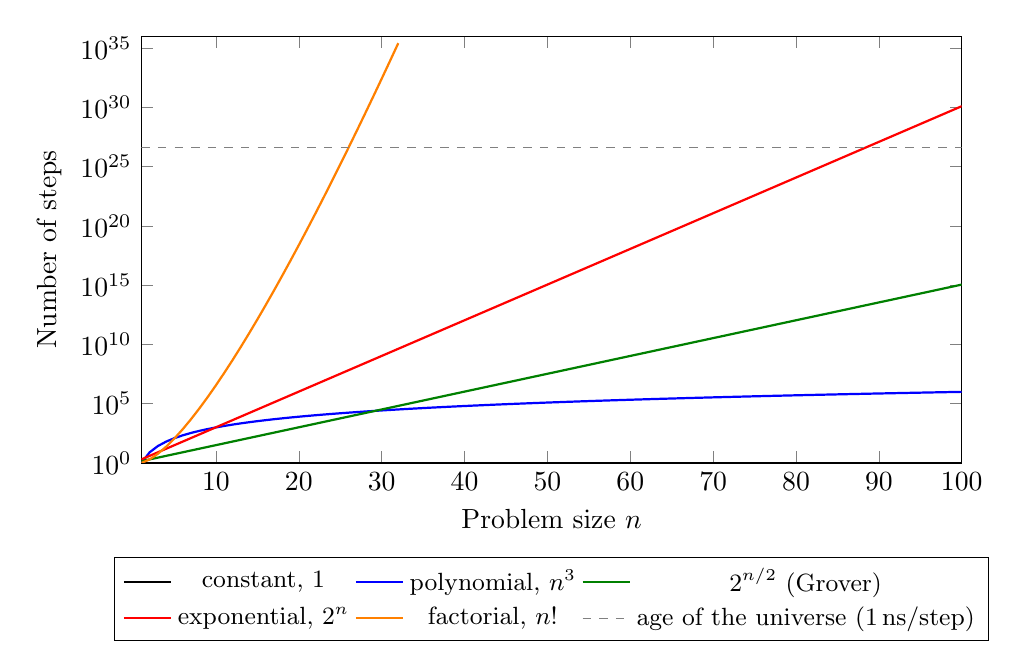
\begin{tikzpicture}
\begin{axis}[width=12cm,height=7cm,ymode=log,xmin=1,xmax=100,ymin=1,ymax=1e36,xlabel={Problem size $n$},ylabel={Number of steps},
  legend style={at={(0.5,-0.22)},anchor=north,legend columns=3,font=\small},ytick={1,1e5,1e10,1e15,1e20,1e25,1e30,1e35}]
\addplot[black,thick,domain=1:100] {1}; \addlegendentry{constant, $1$}
\addplot[blue,thick,domain=1:100,samples=100] {x^3}; \addlegendentry{polynomial, $n^3$}
\addplot[green!50!black,thick,domain=1:100,samples=100] {2^(x/2)}; \addlegendentry{$2^{n/2}$ (Grover)}
\addplot[red,thick,domain=1:100,samples=100] {2^x}; \addlegendentry{exponential, $2^n$}
\addplot[orange,thick] coordinates {(1,1.0000e+00) (2,2.0000e+00) (3,6.0000e+00) (4,2.4000e+01) (5,1.2000e+02) (6,7.2000e+02) (7,5.0400e+03) (8,4.0320e+04) (9,3.6288e+05) (10,3.6288e+06) (11,3.9917e+07) (12,4.7900e+08) (13,6.2270e+09) (14,8.7178e+10) (15,1.3077e+12) (16,2.0923e+13) (17,3.5569e+14) (18,6.4024e+15) (19,1.2165e+17) (20,2.4329e+18) (21,5.1091e+19) (22,1.1240e+21) (23,2.5852e+22) (24,6.2045e+23) (25,1.5511e+25) (26,4.0329e+26) (27,1.0889e+28) (28,3.0489e+29) (29,8.8418e+30) (30,2.6525e+32) (31,8.2228e+33) (32,2.6313e+35)}; \addlegendentry{factorial, $n!$}
\addplot[gray,dashed,domain=1:100] {4e26}; \addlegendentry{age of the universe (1\,ns/step)}
\end{axis}
\end{tikzpicture}
\caption{Number of steps as a function of the problem size $n$, on a logarithmic scale. Polynomial growth appears as a slowly rising curve, exponential growth as a straight line, and factorial growth as an
upward-curving line. The dashed line marks the number of nanoseconds since the Big Bang.}\label{fig:growth}
\end{figure}

\section{Quantum advantage in practice}
The asymptotic classes do not tell the whole story. Constants matter: a quantum gate is $10^3$--$10^6$ times slower than a classical operation, and error correction multiplies the cost further. A quadratic
speed-up therefore pays off only for very long computations: if a classical step takes $1$\,ns and a (logical) quantum step $1\,\mu$s, Grover beats brute force only when $\sqrt N>10^3$, i.e.\ beyond $N\sim10^6$,
and with the overheads of error correction, the cross-over moves to days of computation (Babbush et al., 2021). This is why the most promising applications are those with exponential or large polynomial speed-ups:
factoring and discrete logarithms, and the simulation of quantum systems (chemistry, materials). Experiments claiming ``quantum advantage'' (Google's random-circuit sampling with 53 qubits in 2019, boson sampling with
photons in 2020) address artificial sampling problems, chosen to be hard classically rather than useful, and improved classical algorithms have repeatedly narrowed the gap.

\section{Exercises}
\begin{exercise}
An algorithm needs $n^5$ steps and another $1.1^n$. For which $n$ does the exponential one become slower? Discuss why polynomial is ``tractable'' even if the exponent is large.
\end{exercise}
\begin{exercise}
Estimate the number of Grover iterations needed to search a 128-bit key (AES-128). If each iteration takes $1\,\mu$s, how long does it take? Why is AES-256 considered quantum-safe?
\end{exercise}
